\subsection{Formalizing Einstein: a foundation in Markov process theory} 
\label{sec:ancey2006} 

A significant theoretical development was made in stochastic modeling of the bedload flux by \citet{Ancey2006}. 
They reinterpreted the concepts of \citet{Einstein1950} to develop a new model of the bedload flux expressed as a Markov birth-death processes. 
The motivation for the \citet{Ancey2006} work was a series of experiments: \citet{Bohm2004} measured the bedload flux of glass beads at the outlet of a narrow flume using a percussion sensor, while \citet{Ancey2006} gathered a higher resolution dataset by filming particle motion with a video camera through the plexiglass sidewall of a narrow flume. 
They obtained bedload flux and motion characteristics using image processing. 
Conditions were highly controlled: uniform 6mm diameter glass beads were used as sediment. The flume was 6.5mm wide, so transport was quasi 1D. 
It only occurred in the downstream direction, and experiments were conducted under steady state conditions when the rate of sediment input was matched by the yield at the outlet. 
Despite this idealized level of control, measured fluxes had large fluctuations. 
Instantaneous values were as much as four times mean values. 

The prevalence of large bedload fluctuations even under these idealized laboratory conditions motivated \citet{Ancey2006} to revisit Einstein's assumptions to develop a model of the bedload flux as a random variable. 
The assumptions underlying their model were: 
\begin{enumerate}
\item The sediment system can be characterized using a control volume with a size much larger than the scale of a single grain, similar to \citet{Einstein1950}. A series of volumes as depicted in \ref{fig:yalin} is not necessary.
\item The motion of each grain is independent of every other, and can be characterized as a random succession of motion and rest intervals. 
\item Transitions between motion and rest states are characterized by probabilities per unit time, or rates. 
\item Choosing a particle at random from the system, the possible transitions of that particle are sufficiently determined by its present state, i.e., motion or rest, and knowledge of its complete history of motion/rest transitions does not improve knowledge of its future state. This is the Markov property. 
\end{enumerate}
These assumptions are enough to develop a birth-death model for the bedload flux. 
Within this model, bedload fluctuations are due to variations in the number of moving particles within the control volume. 
As we will see, \citet{Ancey2006} obtained a probability distribution for the bedload flux. 
The mean of this probability distribution is the Einstein-like formula of Yalin \ref{eq:yalinflux}.  
The variance of this distribution is an unambiguous determination of the expected magnitude of bedload fluctuations. 

\subsubsection{Theoretical development: the number of moving particles within a control volume}

Following \citet{Ancey2006} we consider a control volume as in figure \ref{fig:anceygeometry}, and we assume that a particle's dynamics are independent of its history and of the dynamics of all other particles.  
The probability of entrainment or deposition of a particle at each instant only depends on whether a particle is in motion or at rest at that instant. 
Hence, the stochastic dynamics of each particle satisfy the Markov property: it is independent of the past dynamics and only contingent on the current state of the particle. 
Since there are no interactions between particles to take account of, their dynamics, which are random successions between motion and rest states, can be considered separately. 
At the end, bedload transport within the control volume can be understood as the net contributions from all individual particles within it. 

Therefore, we consider an individual particle within the control volume. 
We denote the probability that this particle is in the rest state at some time $t$ by $\pi_0(t)$ and the probability that it is in the motion state by $\pi_1(t)$.
We consider that within a small time interval $\delta t$, if the particle is at rest, the probability for the particle to transition into motion (entrainment) is $\sigma^{-1}\delta t$. Similarly, if the particle is in motion, the probability that it transitions into rest (deposition) is $\tau^{-1}\delta t$. 
Hence $\sigma^{-1}$ is the rate of entrainment of an individual grain, and $\tau^{-1}$ is the rate of deposition. 
Since these rates have dimensions of inverse time, $\sigma$ can be interpreted as a timescale of rest, and $\tau$ can be interpreted as a timescale of motion. 

\begin{wrapfigure}{l}{0.5\textwidth}
  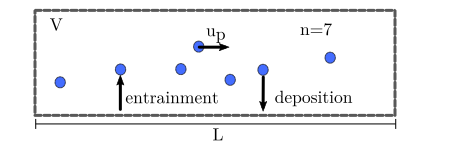
\includegraphics[width=.98\linewidth]{./figures/anceygeometry.png}
  \caption{A control volume $V$ of downstream length $L$ is defined over a region of mobile bed. The number $n$ of particles in motion is considered a random variable due to entrainment and deposition processes. Particles in motion move with velocity $u_p$. \label{fig:anceygeometry}}
\end{wrapfigure}

Using these transition rates and the standard method of setting up a master equation for a birth-death Markov process \citep[e.g.]{Cox1965, Pielou1977, Gillespie1992} develops the following equations describing the flow of probability through time: 
\begin{align} 
\dot{\pi}_0(t) &= \tau^{-1} \pi_1(t) - \sigma^{-1} \pi_0(t) \label{eq:anceymaster2006}\\
\dot{\pi}_1(t) &= \sigma^{-1} \pi_0(t) - \tau^{-1} \pi_1(t).
\end{align}
This two state stochastic process, illustrated in figure \ref{fig:telegraph} is known as the random telegraph process \citep{Gillespie1992, Gardiner1983}, and it is often invoked as a pedagogical example in textbooks on stochastic processes.   

\begin{wrapfigure}{r}{0.25\textwidth}
  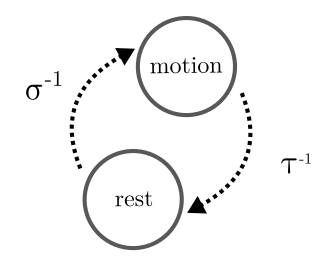
\includegraphics[width=.98\linewidth]{./figures/telegraph.png}
  \caption{Each particle in the control volume switches between motion and rest states with transition rates $\sigma^{-1}$ and $\tau^{-1}$.\label{fig:telegraph}}
\end{wrapfigure}

These equations can be solved for the probability that a particle is at rest -- $\pi_0(t)$ -- or in motion -- $\pi_1(t)$ -- by elementary techniques. 
If the particle is initially at rest, so that $\pi_0(0)=1$ and $\pi_1(0)=0$, the solution is 
\begin{align} \label{eq:anc2006}
\pi_0(t) &=  e^{-t/t_c} + \frac{\tau}{\sigma + \tau}(1-e^{-t/t_c}),\\
\pi_1(t) &= \frac{\sigma}{\sigma + \tau}(1-e^{-t/t_c}).
\end{align}
Here $t_c = \sigma \tau/(\sigma + \tau)$ is a correlation timescale which is the geometric mean of the motion and rest timescales. 
We can see that, after a time $t\gg t_c$, when $e^{-t/t_c} \approx 0$, the trajectory of the particle is independent of (forgets) the initial condition and settles into a stationary state with no time dependence. 
In this steady state, the probability that the particle is in motion is 
\be \pi_1 = \frac{\tau}{\sigma+\tau} = \xi,\ee
while the probability that the particle is at rest is 
\be \pi_0 = \frac{\sigma}{\sigma+\tau} = 1-\xi.\ee

We can interpret $\xi$ as the fraction of time spent in the motion state by the particle on average. 
To see this, we consider the distribution of residence times in the motion state. 
Let $R(T_m)$ be the probability the particle has been in motion for time $T_m$.
Then $R(T_m+\delta t)$ is the probability the particle remains in motion for another period $\delta t$.
This is just the probability the particle was in motion at $T_m$, times the probability that the particle did not deposit in $\delta t$. 
In symbols, $ R(T_m + \delta t) = R(T_m)(1-\tau^{-1}\delta t). $ 
As $\delta t \rightarrow 0$, this develops the differential equation 
\be \frac{d}{dT_m}R(T_m) = -\frac{1}{\tau}R(T_m),\ee
and the solution is the exponential distribution: 
\be R(T_m) = \tau e^{-T_m/\tau}.\ee
Hence the mean time spent in motion is $\tau$. 
By a similar argument, the distribution of resting times is exponential with parameter $\sigma$, so that $\sigma$ is the mean time spent at rest. 
Accordingly $\xi = \tau/(\sigma+\tau)$ represents a fraction of time spent in motion by the particle. 
This is an important link: the parameters $\tau$ and $\sigma$ are observable quantities.
The rate paramters entering the \citet{Ancey2006} model reviewed in this section are summarized in table \ref{tab:symbols2006}. 
\begin{comment}
\begin{wraptable}{r}{0.5\linewidth}
\vspace{-10pt}
\caption{The parameters used in section \ref{sec:ancey2006}}\label{tab:symbols2006}
\begin{tabular}{p{3.3cm}p{3.3cm}}\\
\toprule  
Symbol & Meaning \\
\midrule
$\sigma$ & average time spent at rest \\  
$\mu$ & average time spent in motion\\  
$\xi $ & $\mu/(\sigma+\mu)$ \\ 
\bottomrule
\end{tabular}
\end{wraptable} 
\end{comment} 

We have followed \citet{Ancey2006} to a description of the random start-stop motions of an individual particle. 
The probability that the particle is found in motion is $\xi$ and the probability that it is found at rest is $1-\xi$. 
Hence an observation of whether or not the particle is in motion is a Bernoulli trial with known probabilities, like flipping a coin.
These two probabilities are ratios of observable quantities.  

Now in order to get at the bedload flux, consider that on the bed surface within the control volume there are $N$ particles at any time, each switching randomly from motion to rest as an equilibrium telegraph process. 
We ask, of the $N$ particles, what is the probability that $n$ of them are in motion, $P(n)$?
The sum of $N$ Bernoulli trials is a binomial distribution \citep{Feller1968}, so the probability is
\be P(n) = {N \choose n} \xi^{N-n} (1-\xi)^n \sim \text{Bi}(\xi N, \xi(1-\xi)N). \label{eq:anceybinomial}\ee
This is just the probability that $N-n$ particles are at rest with probability $1-\xi$ while $n$ are in motion with probability $\xi$. 
The factor ${N \choose n}$ represents the number of ways to select the $n$ moving particles from the $N$ total particles.
$\text{Bi}(a,b)$ is a shorthand for a binomial distribution of mean $a$ and variance $b$. 
Hence \citet{Ancey2006} developed a probability distribution for the number of particles in motion in a control volume using the conceptual picture of \citet{Einstein1950}.

Now we outline two important limits of the binomial particle activity distribution as the number $N$ of particles available for motion in the control volume becomes very large.
The first limit is to consider that as $N$ becomes large, the probability $\xi$ that any of these $N$ particles is observed in motion remains fixed. 
In this case, the binomial distribution, equation \ref{eq:anceybinomial}, tends to a Gaussian distribution: 
\be P(n) \sim \mathcal{N}[N\xi, N\xi(1-\xi)]. \label{eq:normaldistflux} \ee
This follows from applying Stirling's formula $\ln(N!) \approx N\ln(N)-N$. 
The second way is to consider that as $N$ becomes large, the probability $\xi$ that any one of these $N$ particles is observed in motion decreases accordingly to leave the product $N\xi \coloneqq \lambda$ fixed. 
Under this limit, the binomial distribution tends to a Poisson distribution: 
\be P(n) \sim \frac{\lambda^n}{n!}e^{-\lambda}. \label{eq:ancey2006poissonlimit}\ee
This follows from taking only the highest order of $N$ from the binomial coefficients, and using one of the definitions of the exponential function: $\lim_{N\rightarrow \infty}(1-\frac{\lambda}{N})^{N} = e^{-\lambda}.$
We will use these limits to evaluate the bedload flux from the particle activity distribution derived in the \citet{Ancey2006} model, and to make contact between this early birth-death model of the bedload flux, and the more sophisticated models which follow it. 

\subsubsection{From the number of moving particles to the bedload flux}
\label{sec:fluxdef}
Usually, the bedload flux is defined as the number of moving particles crossing a surface $S$ perpendicular to the flow direction: $q_s = \int_S \textbf{u}_p \cdot d\textbf{S}$, where $d\textbf{S}$ is an area increment with direction perpendicular to surface $S$ \citep{Ballio2014}.  
The surface $S$ used within the definition of the flux does not have an obvious relationship to the control volume in which we considered the random number of particles in motion. 
We need to connect the properties of bedload motion on a surface to the number of active particles within a volume.  

The surface integral definition of flux just stated is often used in continuum field theories such as classical electrodynamics and kinetic theory, but it is not well suited to discrete particles. 
\citet{Ancey2006} and \citet{Furbish2012} have advocated an alternative formulation based on ensemble averaging. 
This alternative definition hinges on the probability $P[\textbf{u}_p | \textbf{x},t]$ that a particle contacts the control surface $S$ at position $\textbf{x}$ and time $t$ with velocity $\textbf{u}_p$. 
This conditional probability is considered to result from a very large collection of identical systems selected at random moments in their evolution: that is, the conditional probability is an ensemble quantity \citep{Kittel1958}.  

In terms of this ensemble probability, the flux (per unit width) is \citep{Ancey2006}: 
\be q_s = \frac{1}{w}\int_{\text{all } \textbf{u}_p} \int_S P[\textbf{u}_p | \textbf{x},t] \textbf{u}_p \cdot d \textbf{S} d \textbf{u}_p . \label{eq:anceyflux} \ee
I have slightly modified this equation with the factor of $w^{-1}$. 
In steady conditions, when the probability is independent of time -- $\partial P / \partial t = 0$, the ensemble definition of the flux \ref{eq:anceyflux} can be related to the number of moving particles in the control volume we derived in the previous section. 
This link is only approximate, which I believe an under-emphasized point in the literature. 

The approximation is developed by swapping the ensemble interpretation of $P$ by a frequentist interpretation.
This is done by integrating along the control volume.  
If the control volume is sufficiently long, $L \rightarrow \infty$, it can be seen as a stack of very many independent cross sectional surfaces. 
These comprise a stack of replicas of $S$, and at an instant, each surface constitutes one realization (particles intersecting $S$ with some set of positions and velocities) contributing to $P$. 
We can define $P$ by counting occurences along this stack of replica surfaces. 
This becomes an integral across the control volume. 

With this concept of replica surfaces in mind, we can formalize the link with symbols. 
The $n$ particles of radius $a$ will be distributed throughout the volume at some set of positions $\textbf{x}_i$ with some set of velocities $\textbf{u}_i$, where $i=0,1,\dots, n$.
Thus the cloud of particles within the control volume at some instant can be represented by its density in a position-velocity phase space: 
\be \rho(\textbf{x},\textbf{u}_p) = \sum_{i=1}^n M_a(\textbf{x}-\textbf{x}_i)\delta^3(\textbf{u}_p - \textbf{u}_i). \ee  
Here $M_a(\textbf{z})$ is a marker function with definition 
\be 
M_a(\textbf{z}) = 
\begin{cases}
1 & \text{if } |\textbf{z}]< a \\
0 & \text{otherwise}
\end{cases}. 
\ee 
It is $1$ within a sphere of radius $a$ around its argument, and zero otherwise. 
Its volume integral is $\int M_a(\textbf{x}) dV = 4\pi a^3/3 = \nu_p$, the particle volume. 
There are other applications of such functions in \citet{Furbish2012} and \citet{Ballio2014}.

Using this density, for sufficiently large $L$, we can write the conditional probability $P[\textbf{u}_p | \textbf{x}]$ approximately as an integral over the stack of replica surfaces.   
This is an exchange of the ensemble interpretation of $P$ for a frequentist interpretation: 
\be P[\textbf{u}_p|\textbf{x}] \approx \frac{1}{L} \int_0^L dx \rho(\textbf{x},\textbf{u}_p). \ee
The integral runs along the downstream coordinate.
This relationship is only exact as $L \rightarrow \infty$.
Presumably, for fixed $L$, the quality of this approximation would scale with spatial correlations among bedload positions and velocities.
The more correlated bedload positions and velocities are, the worse the approximation will become. 

Using this swap, the bedload flux becomes 
\be q_s \approx \frac{1}{w}\int_{\text{all } \textbf{u}_p} \int_S \frac{1}{L} \int_0^L dx \sum_{i=1}^n M_a(\textbf{x}-\textbf{x}_i)\delta^3(\textbf{u}_p - \textbf{u}_i) \textbf{u}_p \cdot \textbf{k} dS d \textbf{u}_p  = \frac{\nu_p}{Lw} \sum_{i=1}^n \textbf{u}_i\cdot \textbf{k} \ee
It is expressed in terms of the number of particles $n$ within the control volume. $n$ is the random variable we considered earlier as the result of $N$ telegraph processes.
If we write the downstream component of each particle's velocity as $\textbf{u}_i \cdot \textbf{k} = u_{i}$, the bedload flux takes the simple looking form 
\be q_s \approx \frac{\nu_p}{Lw}\sum_{i=1}^n u_i \label{eq:fluxsum} \ee
in terms of the number of particles $n$ within the (necessarily large) control volume and their downstream velocities $u_i$, where $i=1,2,\dots,n$. 
This equation becomes exact as $L\rightarrow \infty$. 

There are options for further analysis of the flux in this way:  
\begin{enumerate}
\item  We can consider the downstream velocities of particles as random variables governed by a probability distribution \citep{Roseberry2012, Furbish2016}, in which case the bedload flux is a sum of a random number $n$ of random variables $u_i$. 
In stochastic processes parlance, a sum of a random number of random variables is called a compound stochastic process \citep{Feller1968}. 
Treating $q_s$ as a compound process has not been fully explored, to my knowledge. 
 
\item We can consider that bedload particles, once set in motion, will all move with approximately the same average velocity, so that the sum \ref{eq:fluxsum} simplifies.
This idea has some theoretical support \citep[e.g.][]{Ancey2003}, although it conflicts with experimental findings \citep{Heyman2016}, so it should be considered critically.  
This is the approach taken by \citet{Ancey2006}.  
\end{enumerate}

For now, we will follow \citet{Ancey2006} to consider that all particles move at approximately the same downstream particle velocity $u_s$, so that the bedload flux becomes 
\be q_s(n) \approx \frac{\nu_p u_s}{Lw} n. \label{eq:fluxy}\ee
The flux is directly proportional to the number $n$ of moving particles within the control volume. 
The bedload flux is a random quantity which inherits its statistical properties from $n$. 

\subsubsection{The bedload flux as a random variable: Einstein revisited, Yalin an intermediary} 

Now we develop the probability distribution of the bedload flux by combining the results we have obtained so far: (1) the probability distribution of the number of moving particles within a control volume equation \ref{eq:anceybinomial}, and (2) the relationship between the number of moving particles and the bedload flux equation \ref{eq:fluxy}. 
Using the law for transformation of discrete random variables \citep[e.g.][]{Feller1968},
\be P(q_s) \approx \sum_{n=0}^N P(n) \delta_{n,Lw q_s/(\nu_p u_s)} ,\label{eq:above}\ee
but this is not valid. 
Since the bedload flux is only approximately given by \ref{eq:fluxy} there is no guarantee that $q_s Lw /(\nu_p u_s)$ will be an integer, and this transform cannot be carried through.  

Instead, we can take advantage of the large $L$ assumption embedded into the equation \ref{eq:fluxy}. 
Because $L$ is necessarily large and $N \propto L$, it follows that $N$ is also large when \ref{eq:fluxy} is valid. 
Therefore, we can also take a limit of the binomial distribution $P(n)$ as the number $N$ of particles in the control volume becomes very large, while the probability that any individual particle is observed in motion remains fixed. 
We can use the resulting distribution, equation \ref{eq:normaldistflux}, with \ref{eq:fluxy}, to derive the bedload flux distribution without the mathematical ambiguity of \ref{eq:above}. 
The probability distribution for the bedload flux becomes, using the law for transformations of continuous random variables \citep[e.g.][]{Feller1968} with \ref{eq:fluxy} and \ref{eq:normaldistflux}:
\be P(q_s) \approx \int_0^\infty dn \delta(n - L w q_s/(\nu_p u_s)) P(n) \approx \mathcal{N}\big(N\xi [\nu_p u_s/(Lw)], N\xi(1-\xi)[\nu_p u_s/(Lw)]^2\big) \label{eq:anceygauss}\ee
\citet{Ancey2006} obtain a normal distribution for the bedload flux. 

Now we discuss the connection of the \citet{Ancey2006} formalism to the earlier work of \citet{Einstein1950}. 
From equation \ref{eq:anceygauss}, the mean flux is 
\be \bra q_s \ket = \nu_p u_s \xi \frac{N}{Lw}.\ee
According to \citet{Einstein1950}, the ratio $N/(Lw)$ is related to the particle size via $N/(Lw) = 1/ a^2$. Since the particle volume is $\nu_p = 4\pi a^3/3$, the mean flux becomes 
\be \bra q_s \ket = \frac{4}{3}\pi a u_s \xi. \ee
Einstein famously considered that the average jump distance of a particle within a single motion interval was proportional to the particle size \citep{Einstein1950, Yalin1972}. 
If we denote the jump distance as $l$ to distinguish it from the control volume size $L$, this means $a \propto l$.
Similarly, Einstein held that the mean transport rate scaled with an inverse characteristic timescale.  
Originally, it was expressed in terms of the particle size and the settling velocity \citep{Einstein1950}. 
Later on, \citet{Yalin1972} concluded it was a timescale of turbulent fluctuations, and there have been similar interpretations by other investigators \citep{Paintal1971, Cheng2004, Armanini2015}. 
Apparently, in this case, to make the link from \citet{Ancey2006} to \citet{Einstein1950}, the timescale should be 
$\tau = k a/u_s$, where $k$ is a constant of proportionality.  
With these substitutions, the bedload flux becomes 
\be \bra q_s \ket = A \frac{a l}{\tau} \xi ,\ee
where $A$ is a constant of proportionality. 
This is similar to Yalin's reinterpretation of Einstein, equation \ref{eq:yalinflux}. 
In the \citet{Ancey2006} model, $\xi$, the fraction of time spent in motion by a single particle, plays the role of $p$, which was the probability of (only) one entrainment in a unit of time.  
In contrast to the $p$ and $\tau$ of \citet{Einstein1950}, the parameters of this model, $\xi$ and $\tau$, are measurable quantities with a clear physical basis. $\xi$ is the fraction of time spent in motion by an individual particle. $\tau$ is the ratio of particle size and the average downstream velocity of sediment in motion.  
We can conclude that \citet{Ancey2006} has reframed and extended Einstein's theory using stochastic mathematics, treating the bedload flux as a statistical quantity. 
The parameters of the refined model have a sound physical interpretation. 

Now we will examine the magnitude of bedload fluctuations expected from the model. 
We can examine the variance of the bedload flux, and compare this to the mean of the flux, to measure the strength of fluctuations. 
However, a clearer conclusion emerges from comparing the mean and variance of the particle activity, derived from the distributions \ref{eq:anceybinomial} or either of its large $N$ limits. 
The ratio of the variance to the mean is 
\be \frac{\bra \delta n^2 \ket}{\bra n \ket} = 1 - \xi. \label{eq:2006flucts} \ee
We conclude that according to the \citet{Ancey2006} model, because $\xi>0$, the variance in the number of active particles within the observation window should never exceed the mean.   

All of the experiments of \citet{Ancey2006} violated this condition, undermining the model, and leading us to examine its assumptions.  
\citet{Ancey2006} hypothesized that the inability of the birth-death model they developed to describe experimental fluctuations was due to the lack of interaction between particles as they transition between motion and rest states. 
They noted that particles preferentially moved in groups, and that the entrainment of one particle led to subsequent entrainment of neighboring particles which were contingent on it for stability. 
Therefore they extended their 2006 model to include a collective motion effect in \citet{Ancey2008}. 
As it turns out, this inclusion leads to a negative binomial distribution of the bedload flux.
This distribution has a sufficiently heavy tail to describe experimental bedload fluctuations. 
We focus on the \citet{Ancey2008} model and the collective entrainment process it introduces in the next section.
 

